%%%%%%%%%%%%%%%%%%%%%%%%%%%%%%%%%%%%%%%%%%%%%%%%%%%%%%%%%%%%%%%%%%%%%%
% LaTeX Example: Project Report
%
% Source: http://www.howtotex.com
%
% Feel free to distribute this example, but please keep the referral
% to howtotex.com
% Date: March 2011 
% 
%%%%%%%%%%%%%%%%%%%%%%%%%%%%%%%%%%%%%%%%%%%%%%%%%%%%%%%%%%%%%%%%%%%%%%
% How to use writeLaTeX: 
%
% You edit the source code here on the left, and the preview on the
% right shows you the result within a few seconds.
%
% Bookmark this page and share the URL with your co-authors. They can
% edit at the same time!
%
% You can upload figures, bibliographies, custom classes and
% styles using the files menu.
%
% If you're new to LaTeX, the wikibook is a great place to start:
% http://en.wikibooks.org/wiki/LaTeX
%
%%%%%%%%%%%%%%%%%%%%%%%%%%%%%%%%%%%%%%%%%%%%%%%%%%%%%%%%%%%%%%%%%%%%%%
% Edit the title below to update the display in My Documents
%\title{Project Report}
%
%%% Preamble
\documentclass[paper=a4, fontsize=11pt]{scrartcl}
\usepackage[T1]{fontenc}
\usepackage{fourier}

\usepackage[english]{babel}															% English language/hyphenation
\usepackage[protrusion=true,expansion=true]{microtype}	
\usepackage{amsmath,amsfonts,amsthm} % Math packages
\usepackage[pdftex]{graphicx}	
\usepackage{url}


%%% Custom sectioning
\usepackage{sectsty}
\allsectionsfont{\centering \normalfont\scshape}


%%% Custom headers/footers (fancyhdr package)
\usepackage{fancyhdr}
\pagestyle{fancyplain}
\fancyhead{}											% No page header
\fancyfoot[L]{}											% Empty 
\fancyfoot[C]{}											% Empty
\fancyfoot[R]{\thepage}									% Pagenumbering
\renewcommand{\headrulewidth}{0pt}			% Remove header underlines
\renewcommand{\footrulewidth}{0pt}				% Remove footer underlines
\setlength{\headheight}{13.6pt}


%%% Equation and float numbering
\numberwithin{equation}{section}		% Equationnumbering: section.eq#
\numberwithin{figure}{section}			% Figurenumbering: section.fig#
\numberwithin{table}{section}				% Tablenumbering: section.tab#


%%% Maketitle metadata
\newcommand{\horrule}[1]{\rule{\linewidth}{#1}} 	% Horizontal rule

\title{
		%\vspace{-1in} 	
		\usefont{OT1}{bch}{b}{n}
		\normalfont \normalsize \textsc{COM SCI 219, Spring 2017, UCLA} \\ [25pt]
		\horrule{0.5pt} \\[0.4cm]
		\huge Checkpoint Report: Cloud-Assited File Sync System  \\
		\horrule{2pt} \\[0.5cm]
}
\author{
		\normalfont 								\normalsize
        J. Jeyakumar, C. Muthappan, P. Rajput, L. Wen\\[-3pt]		\normalsize
        \today
}
\date{}


%%% Begin document
\begin{document}
\maketitle
\section{Project Goal}
In this project, we are going to implement a Dropbox-like file sync system based on cloud. On completion, this system is capable to provide file sharing services across multiple users and devices.  

\section{Overall Design}
The typical workflow of file synchronization using our system is illustrated by the diagram below (Fig.~\ref{fig:design}):
\begin{figure*}[!htbp]
   \centering
   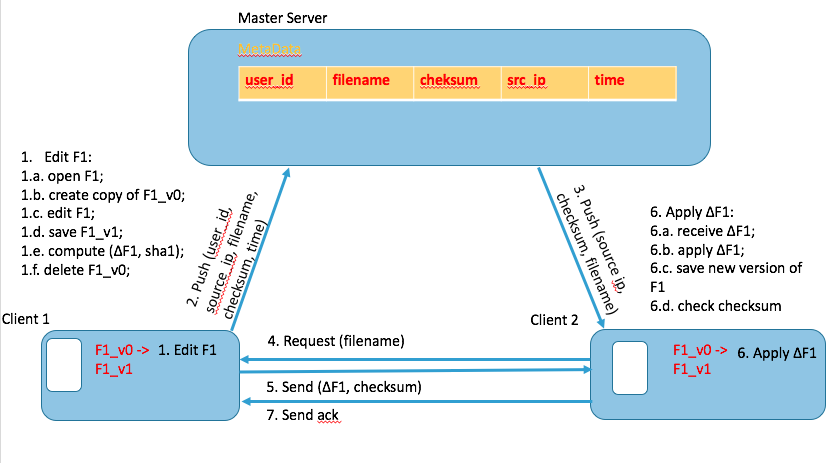
\includegraphics[height=280px, width=400px]{Design_cs219}
   \caption{Overall Design and Typical Workflow}
   \label{fig:design}
\end{figure*}
\subsection{Master Server}
We are going to implement a server side application which will handle all of the meta data. In our preliminary design, a database with columns of user\_id, filename, checksum, src\_ip, timestamp will be maintained on the master server. Each time a client edits a file, it should push the meta-information about the change to the server. Then the server stores the  meta-data and push it to the other connected clients this file is shared with. 
\subsection{Client Device}
On client devices, when connected to the server, every time it receives the meta-information of the changes from the server, it will send a request to the src-ip for the detailed change data. On receiving the data, the client application will apply the changes to the corresponding file, check the validity of the information by computing the checksum, if it is correct, the new version of the file will be saved and the client is supposed to send back the ack message; if not, the file will be rolled back to original version. After ack timeout, the client with src-ip re-sends the packet and the receipt will do this process one more time... This process will go on until the receiver succeeds to apply the correct modifications to the file. 
\section{What is achieved so far?}
\subsection{Server Side}
\subsection{Client Side}
When a file that has to be synced is accessed in a device from any application, our system must be alerted of an incoming change. We achieved this functionality by making use of a python library called pyinotify. This package lets us watch for events that can occur in a directory. These events include many events like CREATE, MODIFY, CLOSE and DELETE. Our approach is very straight forward. When a file in the folder that has to be synced is open by any application in the client, we create a copy of the original version containing the data before modification. When the user closes the file after modification, we find the difference between the new modified file and the old original version.
\section{Difficulties we faced?}
\subsection{Server Side}
\subsection{Client Side}

\section{What is next step?}
\subsection{Server Side}
\begin{itemize}
\item Lock Service\\
    
\item Partitions\\
    Data storage partition.
\end{itemize}

\subsection{Client Side}
%%% End document
\end{document}
